\section{Results}
\label{sec:results}

Figure \ref{fig:main_result} displays the results from the experiments conducted in this project, while Figure \ref{fig:original_result} shows the results from the original paper for comparison. This section examines and contrasts these two sets of results. All experiments were run three times to assess the performance variation of the different ablations. 

\begin{figure}[H]
    \centering
    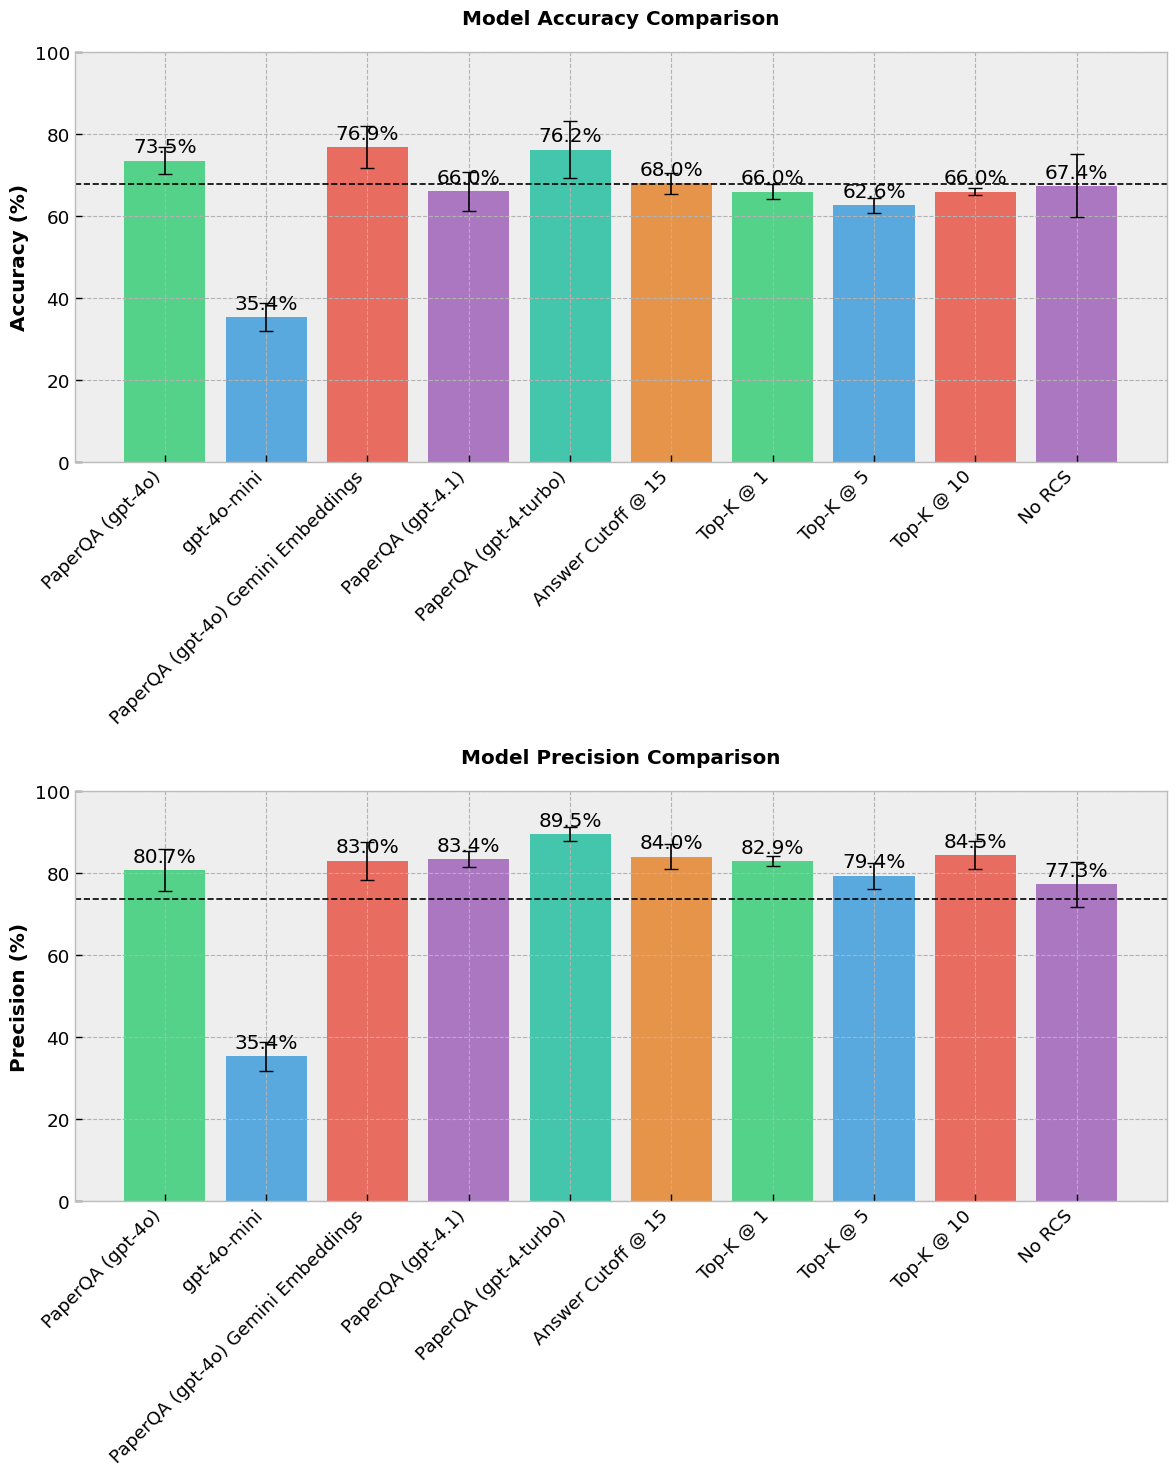
\includegraphics[width=\textwidth]{figures/main_result.png}
    \caption{This project's results against the LitQA test set. Top: Average accuracy of various setups of PaperQA. Bottom: Average precision of the various setups of PaperQA. The dashed line in each plot represents the human benchmark for both accuracy and precision.}
    \label{fig:main_result}
\end{figure}

\begin{figure}[H]
    \centering
    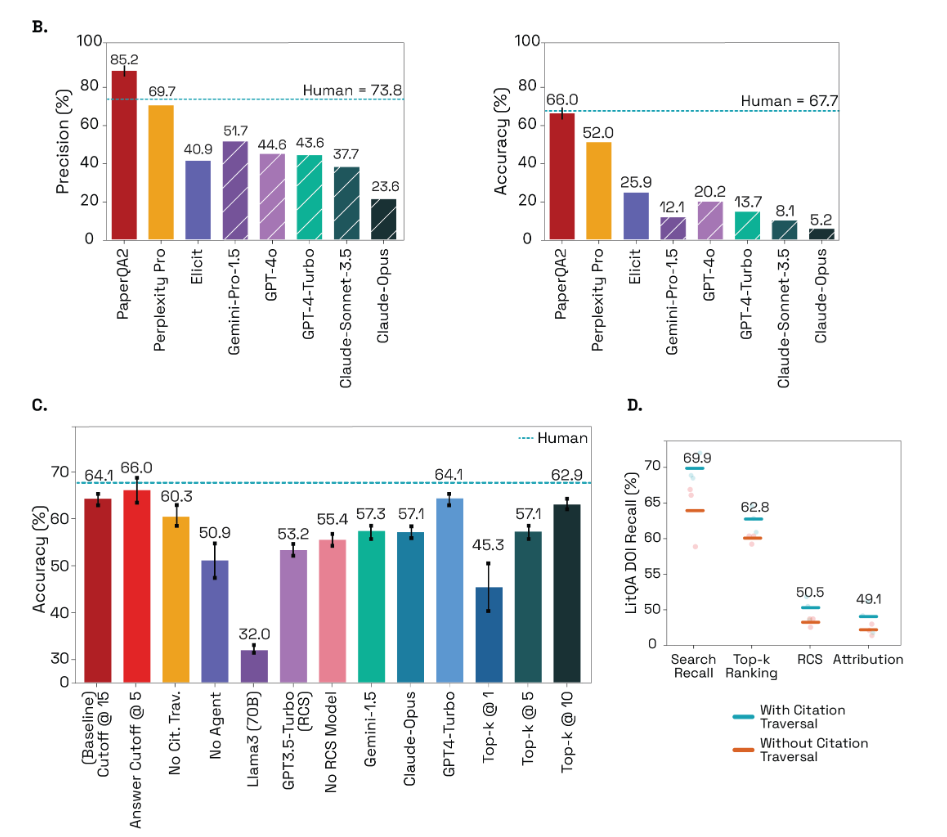
\includegraphics[width=\textwidth]{figures/original_result.png}
    \caption{Original Paper Results. B: Precision and Accuracy of PaperQA and LLMs on LitQA. C: Accuracy of various ablations of PaperQA. D: Aggregated DOI Recall at each stage (This result is not relevant to this report.)}
    \label{fig:original_result}
\end{figure}

\subsection{RAG vs. Standalone LLM}

Consistent with the original study, the results from this project demonstrated that PaperQA outperforms standalone LLMs in question answering. A key difference in behavior was observed: in all standalone evaluations, the LLM attempted to answer every question. Consequently, its accuracy and precision scores were identical, leading to a high rate of hallucination as the model would guess rather than concede an inability to answer. The standalone LLM used in this experiment was \texttt{gpt-4o-mini}, whereas the original paper utilized \texttt{gpt-4-turbo}. The performance of \texttt{gpt-4o-mini} was slightly worse in terms of overall accuracy. 

\subsection{PaperQA Ablations}
The following experiments tested the effect of changing key hyperparameters of PaperQA, from the LLMs used for the agent and RAG components to the top-k retrieval and answer cutoff settings. 

The recreated baseline for PaperQA utilized \texttt{gpt-4o-mini} as the agent and RAG model, with a top-k of 30 and an answer cutoff of 5. The text embedding model was the PaperQA default, \texttt{text-embedding-3-small}. In contrast, the original baseline used \texttt{gpt-4-turbo} for the agent and RAG model, with a top-k of 30 and an answer cutoff of 15. An answer cutoff of 5 was chosen for our baseline, as this was the configuration that achieved 'superhuman' performance in the original study. The recreated baseline appeared to exceed the original, achieving superhuman performance in both accuracy and precision. 

To more closely replicate the original result, an experiment was run using \texttt{gpt-4-turbo} for both the agent and RAG model. The performance was expected to be similar to the original result; however, our experiment achieved superhuman performance in both accuracy and precision. An inspection of the results yielded no evidence of scoring errors that would explain this anomaly. \\

Unexpectedly, using PaperQA with \texttt{gpt-4.1} for both the agent and RAG model resulted in the accuracy dropping to sub-human levels compared to both the original result and our GPT-4-Turbo experiment, with the precision being similar but slightly lower. This was a surprising outcome, as GPT-4.1 is a newer model expected to outperform GPT-4-Turbo across standard benchmarks. 

Across all model variations, the best-performing model in terms of accuracy was the GPT-4o-Mini configuration that used Google's state-of-the-art text embedding model, \texttt{text-embedding-004}. It outperformed the original baseline and consistently achieved superhuman performance in both accuracy and precision. \\

Increasing the answer cutoff had the same effect as in the original paper, decreasing accuracy. However, the effect of removing the RCS step was much less pronounced than in the original study; whereas the original paper reported an accuracy reduction of 12.8\%, our experiment showed a reduction of only 6.1\%.\\

The effect of changing the top-k retrieval setting had a much smaller impact on accuracy compared to the original paper. While the general trend in the original study was that decreasing the top-k value decreased accuracy, our experiments showed no clear correlation. In fact, lowering the top-k to below 10 still yielded near-superhuman accuracy, a level the original paper's configuration (with top-k=30) only narrowly achieved. 

The RCS step was considered crucial for superhuman performance in the original paper, where its removal led to a decrease of around 10\% in accuracy. 
In our recreated experiment, removing the RCS step led to only a 6\% decrease in accuracy, with performance remaining very close to the human benchmark. \\

A key finding is that all experiments involving RAG significantly surpassed the human benchmark for precision, with all ablations achieving at least 77.3\% precision, and the best-performing ablation achieving 89.5\%, exceeding the human benchmark of 73.8\%. \\

The accuracies of the ablations were more varied than the precisions, but this variation was less pronounced than in the original paper. All RAG configurations performed close to or better than the human benchmark, even with hyperparameter settings that were theoretically expected to hinder performance. \\

\textit{It should be noted that an error was discovered in the original accuracy calculation script. Consequently, all accuracy metrics reported herein have been recalculated from the raw outputs to ensure correctness, obviating the need to re-run the experiments.
}





